\documentclass[linenumbers,twocolumn]{aastex631}
% \documentclass[linenumbers]{aastex631}

% Packages
\usepackage[utf8]{inputenc}
\usepackage{graphicx}
\usepackage{amsmath}
\usepackage{amssymb}
\usepackage{enumitem}
\usepackage{ulem}
\usepackage{hyperref}

% Editing commands
\newcommand{\mm}[1]{{\textcolor{purple}{\bf #1}}}

% Make upright subscripts and superscripts in Mathmode.
\def\subinrm#1{\sb{\mathrm{#1}}}
{\catcode`\_=13 \global\let_=\subinrm}
\mathcode`_="8000
\def\supinrm#1{\sp{\mathrm{#1}}}
{\catcode`\^=13 \global\let^=\supinrm}
\mathcode`^="8000
\def\upsubscripts{\catcode`\_=12 } \def\normalsubscripts{\catcode`\_=8 }
\def\upsupscripts{\catcode`\^=12 } \def\normalsupscripts{\catcode`\^=7 }

\newcommand{\vdag}{(v)^\dagger}
\newcommand\aastex{AAS\TeX}
\newcommand\latex{La\TeX}

% Title
\shorttitle{Deriving the Shock Crossing Time}
\shortauthors{Moss M.} 

\begin{document}

\upsubscripts
\upsupscripts

\title{Deriving the Shell Crossing Time as a Function of the Density}

\correspondingauthor{Michael Moss}
\email{mikejmoss3@gmail.com}

\begin{abstract}
The goal of this derivation to estimate the time it will take a reverse shock to cross incoming ejecta material.

\end{abstract}

\section{Introduction}
{
    In the refreshed shock model, the wind of a GRB can be separated into two regions, (i) early outflow launched with $\bar{\Gamma}\sim100$ and (ii) later ejecta launched launched with $\bar{\Gamma}\sim10$. The early material is responsible for producing the prompt emission and the afterglow continuum emission. The later ejecta will eventually catch up to the early ejecta as it sweeps up circumburst medium and decelerates. When the later ejecta catches up and collides with the early material, a ``refreshed'' shock occurs, injecting energy into the front of the outflow and may be witnessed as bumps in the afterglow light curves (potentially in the optical regime). In this work, we would like to estimate the time it takes the incoming energy injected from the later ejecta to be distributed across the newly shocked material. This timescale should be dominated by the shell crossing time $\Delta t_{shell}$, where we model the incoming late ejecta as a shell with mass $M_{r}$ and Lorentz factor $\Gamma_{r}$.

    % \begin{figure*}[t!]
    %     \centering
    %     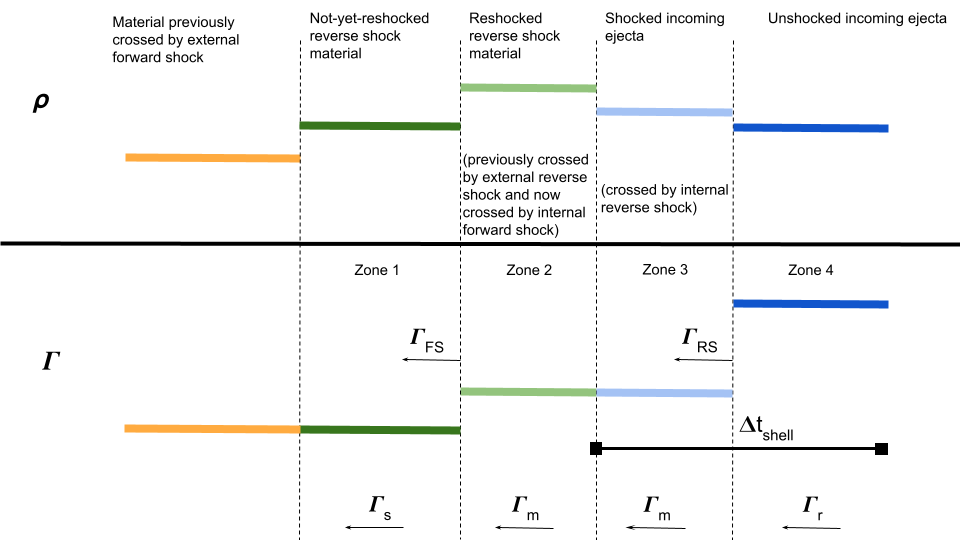
\includegraphics[width=0.8\textwidth]{schematic.png}
    %     \caption{Schematic of the scenario (in the central engine frame). There are two ``reverse shocks'' in question. The reverse shock arising from the bulk of the jet decelerating as it sweeps up circumburst medium, which will be referred to as the external reverse shock. And an internal revers shock arising from the deceleration of the incoming later ejecta decelerating as it rams the material in front of it (which happens to be the material previously crossed by the external reverse shock).}
    %     \label{fig: schematic}
    % \end{figure*}

    To estimate the time it will take for an internal reverse shock to cross incoming material, we must estimate the density in the slow material (zone 1 material) and the rapid material (zone 4 material). 
}

\section{Estimating Density of Relativistic Shell, n4}
{
    The average mass density of the material, $\rho$, in the bulk GRB outflow (in the central engine frame) can be found using the isotropic equivalent energy injection rate, $\dot{E}_{iso}$, 

    \begin{align}
    \dot{E}_{iso} &= \dot{M}_{iso} \bar{\Gamma} c^2\\
    &\text{where } \dot{M}_{iso} = 4 \pi c R^2 \rho\\
    \Rightarrow \rho &= \frac{\dot{E}_{iso}}{4\pi \Gamma_{s,0} c^3 R^2}
    \end{align}

    where $R$ is the distance of the material from the central engine, $\dot{M}_{iso}$ is the isotropic equivalent mass injection rate, and $\bar{\Gamma}$ is the average bulk Lorentz factor of the ejecta. We can estimate the density using the fiducial values $\dot{E}_{iso} = 10^{52}$ erg/s, $R=10^{17}$ cm, and $\bar{\Gamma} = 15$ (since we are considering slow material for the late ejecta), which results in a density of $\bar{\rho}\approx 2\times10^{-16}$ g cm$^{-3}$ ($n \approx 1\times 10^{8}$ cm$^{-3}$; central engine frame). This is very uncertain and most likely a large underestimation of the true density in the merging material. Placing this into the fluid frame requires a factor of $1/\bar{\Gamma}$ such that, $\bar{\rho}'\approx 1\times10^{-17}$ g cm$^{-3}$ ($n' \approx 8\times 10^{6}$ cm$^{-3}$; fluid frame)
}

\section{Estimating the Shell Crossing Time}
{
    Following Sari and Piran 1995 (hereafter SP95)    

    \begin{align}
        \Delta &= ??????????
        % & =?= \frac{R}{\Gamma_2^2} \text{ (Eq 11 of S+P95)}\\
        % & =?= \frac{E_{iso}}{\pi R^2 m_p c^2 n_4}\\
        % & =?= \left(\frac{3 E_{iso}}{4\pi \gamma_4 m_p c^2 n_4}\right)^{1/3}\\
        % & =? = \frac{R_{\Delta} n_1 m_p c^2}{E_{iso}}
    \end{align}, the time it takes an incoming relativistic shell to be crossed by a reverse shock is given by the expression, 

    \begin{align}
        t_{\Delta} = \frac{\Delta}{c(\beta_4 - \beta_2)} \left(1-\frac{\gamma_4 n_4}{\gamma_3 n_3}\right)
    \end{align} 

    where $\beta_i = \sqrt{1 - 1/\gamma_i^2}$ and $\Delta$ is the width of the shell and can be approximated as, 

    \begin{align}
        \Delta &= ??????????
    \end{align}

    \mm{How in the world can I estimate $\Delta$?}

    The shell crossing time depends on the density ratio of the ISM density and the incoming shell, i.e., $f = n_4/n_1$. If $\gamma_4^2 \gg f$, the we are in a relativistic regime and the shell crossing time can be expressed as 

    \begin{align}
        t_{\Delta} = \Delta \gamma_4 \frac{\sqrt{f}}{2c}
    \end{align}

    Alternatively, if $f\gg\gamma_^2$, then the reverse shock is in a Newtonian regime and the shell crossing time is expressed as

    \begin{align}
        t_{\Delta} = \sqrt{\frac{9}{14}}\Delta\gamma_4\frac{\sqrt{f}}{c}
    \end{align}

    \begin{figure}[t!]
        \centering
        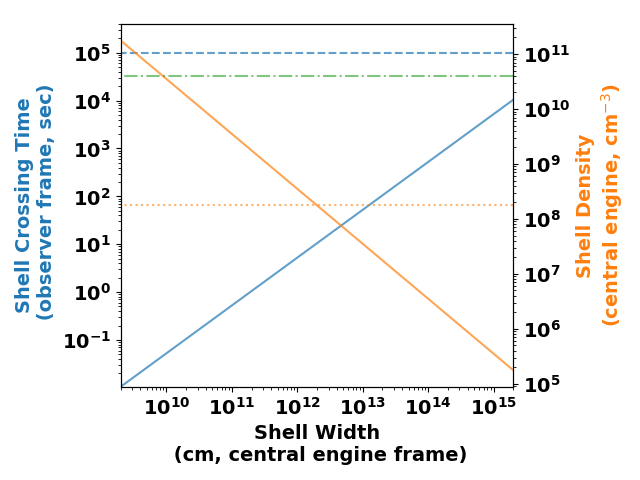
\includegraphics[width=0.45\textwidth]{shell-cross-time.png}
        \caption{Shell crossing time as a function of the density of the material. The estimated density (which is likely an underestimate) is shown by the orange, dashed line. Assuming an ISM density of $n_1 = 1$ cm$^{-3}$, the density at which the collision transitions from Newtonian to relativistic is $\sim 7.8\times10^6$ cm$^{-3}$, shown by a gray, dashed line.}
        \label{fig: plot}
    \end{figure}
}

\section[Estimating The Width of The Relativistic Shell]{Estimating $\Delta$}
{
    SP95 state several example values for the width of the relativistic shell $\Delta$ throughout the text, but these range from $10^7$ cm to $10^{13}$ cm (which directly changes the shell crossing time by six orders of magnitude as well). For the numerical estimates below I assume that $E_{iso}=10^{53}$ erg, $R_{coll} = 10^{17}$ cm, $n_1 = 1$ cm$^{-3}$, and $\gamma_4 = 15$.

    Within the text of the of SP95 it is stated that $R \lesssim \Delta \gamma_4^2$, so maybe

    \begin{align}
        \Delta &=?= R / \gamma_4^2 \\
        &\sim4\times10^{14}\text{ cm} \nonumber
    \end{align}

    This is further supported by M\'eszaros and Rees 1993 Alternatively, within the Spherical Considerations section of SP95, the radius at which the reverse shock crosses the shell $R_{\Delta}$ can be defined as $R_{\Delta} = l^{3/4}\Delta^{1/4}$, where $l=(E/n_1 m_p c^2)$ is the Sedov length, such that

    \begin{align}
        \Delta &=?= \frac{R_{\Delta} n_1 m_p c^2}{E_{iso}} \\
        &\sim1.5\times10^{12}\text{ cm} \nonumber
    \end{align} 

    Is $R_{\Delta}$ the same as the radius of collision? If so, $R_{\Delta}\sim10^{17}$ cm.

    Lastly, I tried to estimate the radius of the outflow by taking the (isotropic) average particle density

    \begin{align}
        \Delta &=?= \left(\frac{3 E_{iso}}{4\pi \gamma_4 m_p c^2 n_4}\right)^{1/3}
    \end{align}

    But, to be more realistic, I am interested in the \textit{shell} of material, not the sphere, so I define $\Delta = R-r$. This allows us to write the volume as $V = 4\pi/3 (R^3- r^3) = 4\pi/3 (R^3- (R-\Delta)^3)$ and the above equation becomes 

    \begin{align}
        \Delta &=?= R - \left(R^3 - \left(\frac{3 E_{iso}}{4\pi \gamma_4 m_p c^2 n_4}\right)\right)^{1/3}
    \end{align}

    Note, this last method allows us to estimate the width of the relativistic shell as a function of the density in the shell. 

    All of the above methods provide estimates that are on the high end of the range of values given in SP95. Furthermore, SP95 state that there is an upper limit of $\Delta < 3\times 10^{12}$ cm (based on the observed durations of the brightest GRBs).
}

\end{document}
